\documentclass[b5paper,opensource]{./template/qyxf-book}

\usepackage{subcaption}
% 添加水印的宏包
\usepackage{draftwatermark}
\SetWatermarkText{钱院学辅}
\SetWatermarkLightness{0.9}
\SetWatermarkScale{0.9}

% 基本不需要改动
\title{大物题解}
\subtitle{Key to Universal Physics}
\author{钱院学辅大物编写小组}
\typo{钱院学辅排版组}
\date{\today}
\version{v1.0}
\sourcepage{\url{https://github.com/qyxf/Tutorials/}}

% 这里可以自定义一些命令
\newcommand{\di}[1]{\mathrm{d}#1}
\newcommand{\p}[2]{\frac{\partial #1}{\partial #2}}
\newcommand{\pp}[2]{\frac{\partial ^2 #1}{\partial #2 ^2}}
\newcommand{\dy}[2]{\frac{\di{#1}}{\di{#2}}}
\newcommand{\ddy}[2]{\frac{\mathrm{d} ^2 #1}{\mathrm{d} #2 ^2}}
\newcommand{\zbj}[4]
{
	\draw (0,0) node[below left] {$ O $};
	\draw [->] (#1,0) -- (#2,0) node[right] {$ x $};
	\draw [->] (0,#3) -- (0,#4) node[right] {$ y $};
}


\begin{document}
\chapter{磁场1}  % 使用章节\chapter{}来做一级标题
\section{选择题}  % 选择题、填空题和解答题使用\section{}

\exercise{1}D  % 题号使用这个命令,会自动生成标记,注记后写主要答案

\solve
由毕奥萨法尔定律,$B=\int\frac{\mu_0I}{4\pi}\frac{\di l}{R^2}$,而$\int\di l=\pi R$,所以,$B=\frac{\mu_0I}{4R}$.

\exercise{2}C

\solve
根据毕奥萨法尔定律,载流直导线在电流方向的延长线上产生的磁感应强度为0,故$B_1=0$;而由环路定理,无限长载流直导线在距它距离为$a$处产生的磁感应强度为$B\cdot2\pi a=\mu_0I$,本题中半无限长载流直导线产生的磁感应强度恰好为无限长在流直导线的一半,故$B_2=\frac{\mu_0I}{4\pi a}$.所以,$O$点处
\begin{equation*}
B=B_1+B_2=0+\frac{\mu_0I}{4\pi a}=\frac{\mu_0I}{4\pi a}
\end{equation*}

\exercise{3}A

\solve
首先分析电路,$acb$段电阻为$ab$段电阻的两倍,故流过$ab$段的电流为$I_{ab}=\frac{2}{3}I$,流过$acb$段的电流为$I_{acb}=\frac{1}{3}I$.再判断产生的磁场方向,$ab$段在$O$点处产生的磁感应强度方向垂直纸面向外,$acb$段产生的磁感应强度方向垂直纸面向里,再根据对称性,$B_{ab}=-2B_{ac}=-2B_{cb}$,所以$B_{ab}+B_{acb}=B_{ab}+2\cdot(-\frac{1}{2}B_{ab})=0$;$O$点位于1段电流的延长线上,故$B_1=0$;下面只需计算2段电流在$O$点处产生的磁感应强度大小,设$O$点距离$bc$边的垂直距离为$a=\frac{\sqrt{3}d}{6}$,则根据直导线的磁感应强度公式$B_2=\frac{\mu_0I}{4\pi a}(\cos 0-\cos\frac{\pi}{6})=(\frac{\sqrt{3}}{2}-\frac{3}{4})\frac{\mu_0I}{\pi d}$.综上,$O$点处$B=B_{ab}+B_{acb}+B_1+B_2=(\frac{\sqrt{3}}{2}-\frac{3}{4})\frac{\mu_0I}{\pi d}$.

\exercise{4}C

\solve
边长为$a$的正方形各边距中心点的距离为$\frac{a}{2}$,所以根据直导线的磁感应强度公式,$B=\frac{\mu_0I}{4\pi\cdot\frac{a}{2}}(\cos\frac{\pi}{4}-\cos\frac{3\pi}{4})=\frac{\sqrt{2}\mu_0I}{2\pi a}$.

\exercise{5}B

\begin{figure}[htbp]  % 可以使用figure来导入图片
	\centering
	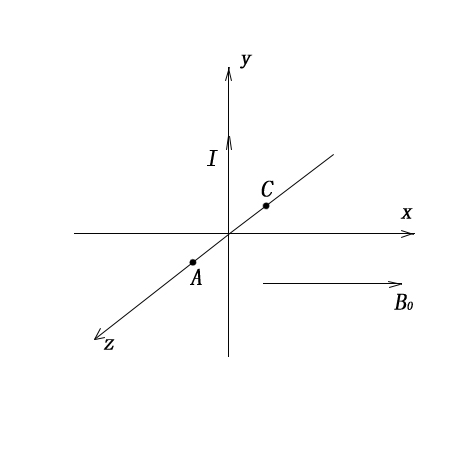
\includegraphics[width=15em, height=15em]{Chp8_illus1.jpg}
	\caption{练习5}
	\label{fig:c1}
\end{figure}

\solve
如图\ref{fig:c1},电流$I$在$AC$两点产生的磁感应强度为$B_1=\frac{\mu_0I}{2\pi\cdot2}=10^{-6}T$,在$A$处方向为$x$轴正向,在$C$处方向为$x$轴负向;所以,$A$点处$B_0$与$B_1$叠加后的$B_A=2\times10^{-6}T$,$C$点处$B_0$与$B_1$叠加后的$B_C=0$.

\exercise{6}B

\solve
磁矩$\mu=i\cdot S$,边长扩大3倍,面积扩大9倍,磁矩扩大9倍.

\exercise{7}A

\begin{figure}[htbp]  % 可以使用figure来导入图片
	\centering
	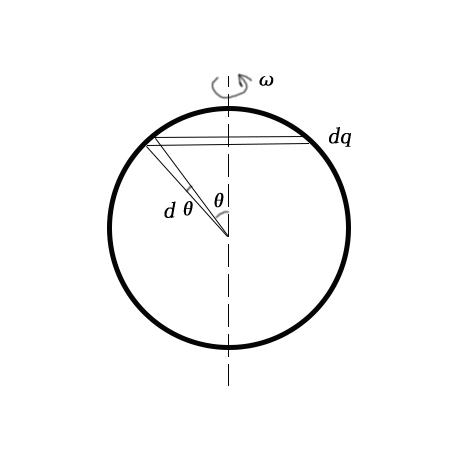
\includegraphics[width=15em, height=15em]{Chp8_illus2.jpg}
	\caption{练习7}
	\label{fig:c2}
\end{figure}

\solve
如图\ref{fig:c2}所示,取$\di\theta$的微元,所以$\di q=2\lambda R\di\theta$,所以电流微元$\di I=\frac{\di q}{t}=\frac{2\lambda R\di\theta}{\frac{2\pi}{\omega}}=\frac{\lambda\omega R\di\theta}{\pi}$,磁矩微元$\di\mu=\di I\cdot S=\frac{\lambda\omega R\di\theta}{\pi}\cdot\pi(R\sin\theta)^2=\lambda\omega R^3\int_0^\pi\sin^2\theta\di\theta=\frac{\pi\lambda\omega R^3}{2}$.

\exercise{8}B

\solve
根据安培环路定理可得$B\cdot 2\pi r=\mu_0I$,代入数据计算出$I=1.4$A.

\exercise{9}B

\solve
环路$L$所围的电流$\sum I=0$,所以$\oint_L\vec{B}\cdot\di\vec{l}=0$,但环路$L$上每一点的磁感应强度$B$均垂直于环路$L$,故任一点$B\ne0$.

\exercise{10}C

\solve
竖直摆放的导线1在$M$、$N$点处产生的磁感应强度方向垂直纸面向里,记为$B_1$,水平摆放的导线2在$M$处产生的磁感应强度垂直纸面向里,在$N$处产生的磁感应强度垂直纸面向外,大小记为$B_2$;故$B_M=B_1+B_2$,$B_N=B_1-B_2$,即有$B_M>B_N$.

\section{填空题}
\exercise{11} 0

\analysis
根据空间位置关系,线圈$abcd$绕$cd$边旋转60°角后,恰好全部离开磁场,所以磁通为0.

\exercise{12} 0

\analysis
由对称性,$ab$间的每一条导线上的电流均为$\frac{I}{4}$,每一个半圆环在环中心处产生的磁感应强度恰好与与之相对的半圆环在环中心处产生的磁感应强度大小相等,方向相反,四个圆环相叠加后环中心处总的磁感应强度为0.

\exercise{13} 1:1

\solve
由无限长直导线的磁感应强度公式可知,$B=\frac{\mu_0I}{2\pi r}$.所以,设$S_1$和$S_2$的宽度均为$l$,$\Phi_1=\int_a^{2a}B(r)l\di r=\frac{\mu_0Il}{2\pi}\ln2$,$\Phi_2=\int_{2a}^{4a}B(r)l\di r=\frac{\mu_0Il}{2\pi}\ln2$,比值为1:1.

\exercise{14} $\frac{\mu_0I}{4R}\vec{i}+\frac{\mu_0I}{2\pi R}\vec{k}$

\solve
$yOz$平面上的半圆环在$O$点产生的磁感应强度为$\vec{B_1}=\frac{\mu_0I}{4R}\vec{i}$,两条半长直导线在$O$点处产生的磁感应强度为$\vec{B_2}=2\cdot\frac{\mu_0I}{4\pi R}\vec{k}$,所以总磁感应强度为$B=\frac{\mu_0I}{4R}\vec{i}+\frac{\mu_0I}{2\pi R}\vec{k}$


\exercise{15} 1

\analysis
无限长载流螺线管内的磁感应强度大小为$B=\mu_0nI$,式中,$n$为单位长度上的匝数,$I$为通过导线的电流,故无限长载流螺线管在管内的磁感应强度与螺线管的半径无关,所以$\frac{B_R}{B_r}=1$.

\exercise{16} $\frac{\mu_0ih}{4\pi^2R^2}$

\solve
首先在狭缝处补上一个宽度为$h$,电流为$I=\frac{h}{2\pi R}i$的电流,则将原无限长导体薄管凑成了一整个无限长导体薄管,根据对称性,这个无狭缝的无限长导体薄管在其轴线上产生的磁感应强度为0;再在原狭缝处补上一个宽度为$h$,电流为$I=-\frac{h}{2\pi R}i$的电流,这一电流在管轴线上产生的磁感应强度大小为$B=\frac{\mu_0ih}{4\pi^2R^2}$即为管轴线处实际的磁感应强度大小.

\exercise{17} $4\pi\times10^{-6}$


\solve
密绕细长直螺线管在管内产生的磁场为匀强磁场,其磁感应强度为$B=\mu_0nI=4\pi\times10^{-7}\cdot\frac{10}{0.01}\cdot10=4\pi\times10^{-3}T$,磁通为$\Phi=BS=4\pi\times10^-3\cdot10\time10^{-4}=4\pi\times10^{-6}Wb$.

\exercise{18} $\frac{\mu_0I}{4\pi R}$

\solve
长直导线1在$O$点处产生的磁感应强度为$0$;流过$ab$劣弧的电流为$\frac{3}{4}I$,流过$ab$优弧的电流为$\frac{1}{4}I$,再次根据对称性,可知$ab$劣弧和$ab$优弧在$O$点处产生的磁感应强度和为0;最后只剩下长直导线2,它在$O$点处产生的磁感应强度$B=\frac{\mu_0I}{4\pi R}$即为$O$点处的磁感应强度大小.

\exercise{19} $\frac{\sqrt{2}\mu_0I\di l}{16\pi}$\quad z轴正向

\solve
电流元$I\di\vec{l}$距离$P$点的距离为$\sqrt{2}$,由毕奥萨法尔定律,$P$点处
\begin{equation*}
\di B=\frac{\mu_0}{4\pi}\cdot\frac{I\di l\cdot\sin\frac{3\pi}{4}}{2}=\frac{\sqrt{2}\mu_0I\di l}{16\pi}
\end{equation*}

\exercise{20} 0\quad$-\mu_0 I$

\analysis
$A$与$B$在$P$点产生的磁感应强度大小相等,方向相反,故$B_p=0$.如题图所示环路方向,结合安培环路定理可知$\oint_L\vec{B}\cdot\di\vec{l}=-\mu_0 I$.

\section{计算题}
\exercise{21}

\solve
在圆盘上取半径从$r$到$r+\di r$的一个圆环微元.

这个圆环微元产生的等效电流大小为
\begin{equation*}
i=\frac{q}{t}=\frac{2\pi r\di r\cdot\sigma}{\frac{2\pi}{\omega}}=\sigma\omega r\di r
\end{equation*}
所以,这个圆环微元在盘心产生的磁感应强度为
\begin{equation*}
\di B=\frac{\mu_0}{4\pi}\cdot\frac{i\cdot2\pi r}{r^2}=\frac{\mu_0i}{2r}=\frac{1}{2}\mu_0\sigma\omega\di r
\end{equation*}
所以
\begin{equation*}
B=\int_0^R\di B=\int_0^R\frac{1}{2}\mu_0\sigma\omega\di r=\frac{1}{2}\mu_0\sigma\omega R
\end{equation*}
方向与$\vec{\omega}$相同.

\exercise{22}

\solve 
由对称性,平面$y=0$上$B=0$,且磁场在$\vec{k}$方向上的分量大小为$0$.

取一个与$xOy$面平行的环路,其一边在$y=0$的平面上,另一边在$y=y$的平面上,宽为$l$.

由安培环路定理,当$|y|\le d$时,有
\begin{equation*}
B(y)\cdot l=\mu_0\sigma ly
\end{equation*}
当$|y|>d$时,有
\begin{equation*}
B(y)\cdot l=\mu_0\sigma ld
\end{equation*}
所以
\begin{equation*}
B(y)=
\begin{cases}
\mu_0\sigma|y|\qquad|y|\le d\\
\mu_0\sigma d\qquad|y|>d
\end{cases}
\end{equation*}
当$y>0$时,方向沿$x$轴负向;当$y<0$时,方向沿$x$轴正向.

\exercise{23}

\solve
对于半径为$R$的大圆环来说,记在距其环心距离为$x$处的磁感应强度为$B(x)$
\begin{equation*}
B=\frac{\mu_0IR^2}{2(R^2+x^2)^{\frac{3}{2}}}
\end{equation*}
由题目假设$x\gg R$,所以$B(x)=\frac{\mu_0IR^2}{2x^3}$

又有$x\gg R\gg r$,所以可近似视半径为$r$的圆环处磁感应强度为一常数.综上,小线圈中的磁通量为
\begin{equation*}
\Phi=B\cdot S=\frac{\mu_0IR^2}{2x^3}\cdot \pi r^2=\frac{\pi\mu_0Ir^2}{2k^3R}
\end{equation*}

\exercise{24}

\solve
在$O'$处填补与$I$方向、密度均相同的电流$I_1$和与$I$方向相反、密度相同的电流$I_2$
\begin{equation*}
I_1=I_2=\frac{I}{\pi (R_1^2-R_2^2)}\cdot\pi R_2^2=\frac{R_2^2}{R_1^2-R_2^2}I
\end{equation*}

(1)由对称性,圆柱体$O$与填补上的$I_1$在圆柱体轴线上产生的$B=0$.只需考虑在$O'$处填补的电流$I_2$电流.

由安培环路定理$B_1\cdot2\pi b=\mu_0I_2$,所以
\begin{equation*}
B_1=\frac{\mu_0I}{2\pi b}\cdot\frac{R_2^2}{R_1^2-R_2^2}
\end{equation*}

(2)$I_2$在$O'$处轴线上产生的$B=0$,则只需考虑在$O$处的大圆柱电流产生的磁场即可.

由安培环路定理$B_2\cdot2\pi b=\mu_0\frac{I}{R_1^2-R_2^2}b^2$,所以
\begin{equation*}
B_2=\frac{\mu_0I}{2\pi}\cdot\frac{b}{R_1^2-R_2^2}
\end{equation*}
\end{document}